\chapter{Naître, grandir, mourir}\label{ch:g2:born-grow-die}

Au printemps, le cerisier près du portail est couvert de \omterm{def:g1:plants-around-us:parts}{fleurs}~;
dessous, une chatte allaite ses chatons nouveau-nés~; et papi montre
une photo de lui quand il avait ton âge --- petit, les dents
écartées, et déjà amateur de cerises. Tout \omterm{def:g1:living-or-not:living}{être vivant} suit la même
route~: il commence, il grandit, et un jour il finit. Cette route
s'appelle le \omterm{def:g2:born-grow-die:cycle}{cycle de vie}.

\section{Les étapes d'une vie}

\begin{definition}[Cycle de vie]\label{def:g2:born-grow-die:cycle}
Le \emph{cycle de vie}\index{cycle de vie} d'un \omterm{def:g1:living-or-not:living}{être vivant} est la
suite des \emph{étapes}\index{étape} que sa vie traverse~:
\begin{enumerate}
  \item il \emph{naît}\index{naissance} --- le commencement~;
  \item il est \emph{jeune}\index{jeune} --- il grandit et change
        vite~;
  \item il est \emph{adulte}\index{adulte} --- entièrement
        grandi~; les adultes peuvent avoir des petits~;
  \item il devient \emph{vieux}\index{vieillesse}, et à la fin il
        \emph{meurt}\index{mort}.
\end{enumerate}
\end{definition}

\begin{example}[Trois vies, une même route]\label{ex:g2:born-grow-die:three}
Un chaton naît, joue et devient un chat, qui aura peut-être des
chatons à son tour, et vieillit. Un noyau de cerise germe, le jeune
arbre grandit pendant des années, l'arbre \omterm{def:g2:born-grow-die:cycle}{adulte} donne des \omterm{def:g1:plants-around-us:parts}{fleurs} et
des cerises, et après plusieurs dizaines d'années il meurt. Et toi~:
bébé, enfant, puis un jour \omterm{def:g2:born-grow-die:cycle}{adulte}. Chaton, cerisier, enfant --- les
mêmes quatre \omterm{def:g2:born-grow-die:cycle}{étapes}.
\end{example}

\begin{omfigure}
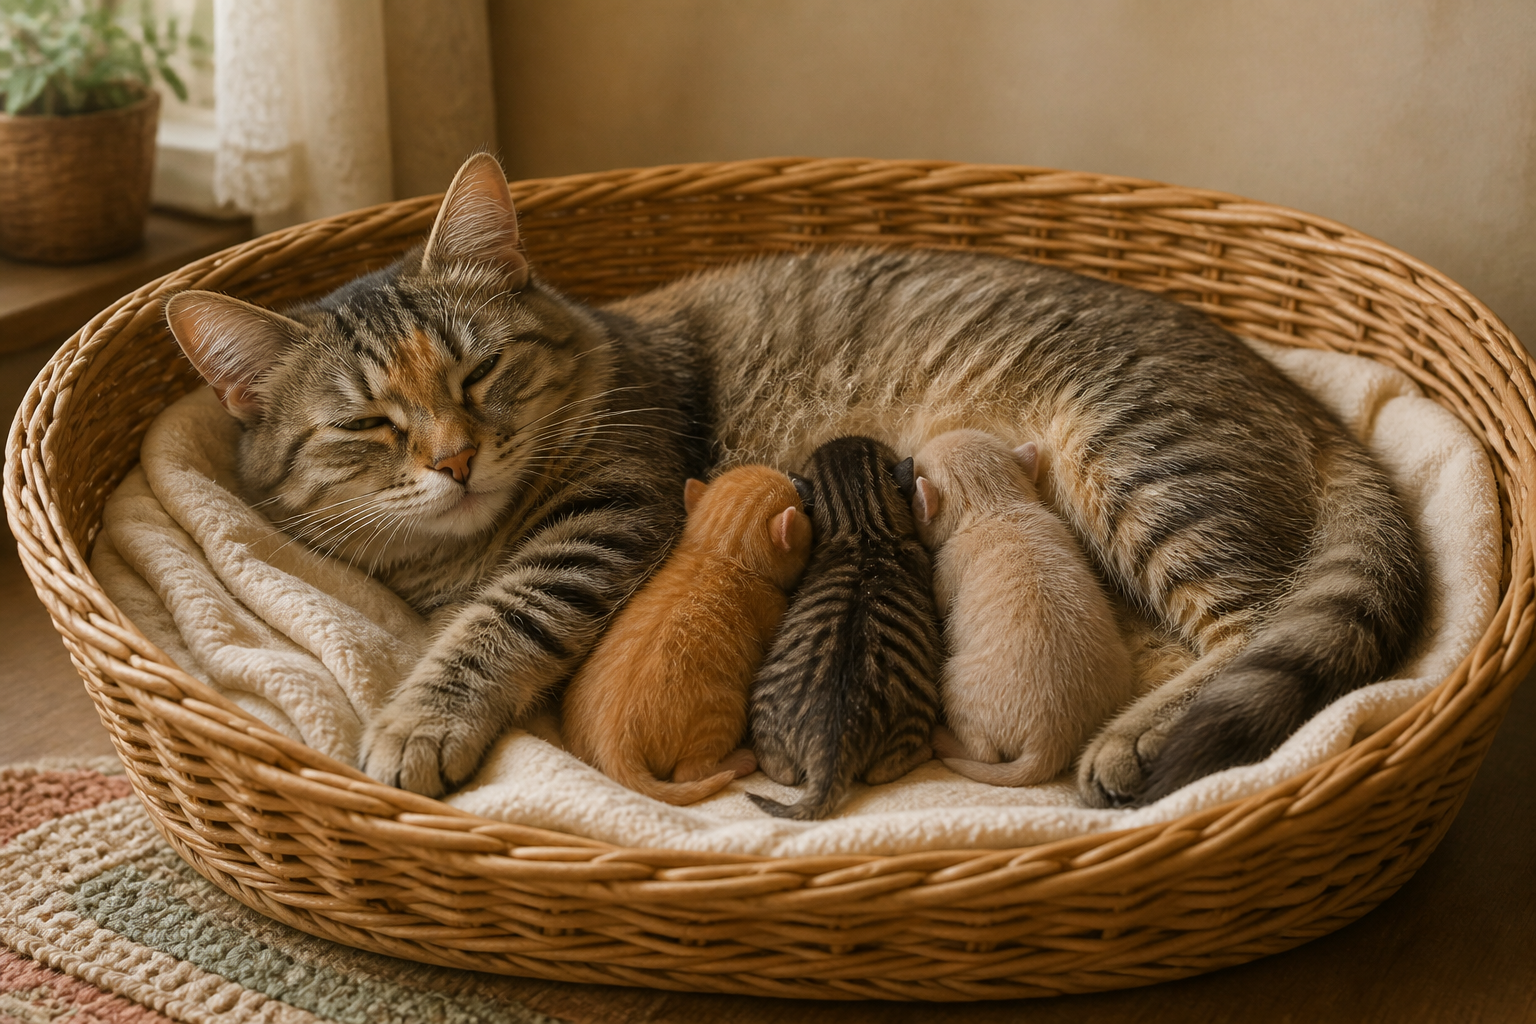
\includegraphics[width=0.62\linewidth]{images/book1/ai/g2-cycle-kittens.png}

{\small Le début de trois \omterm{def:g2:born-grow-die:cycle}{cycles de vie} à la fois~: des chatons
nouveau-nés au lait de leur mère.}
\end{omfigure}

\begin{omfigure}
\begin{tikzpicture}[scale=0.92]
  \foreach \x/\txt in {0/{naissance},3.1/{jeune},6.2/{adulte},9.3/{vieillesse}} {
    \draw[thick, omDef, fill=omDef!7, rounded corners=5pt]
      (\x,0) rectangle ({\x+2.4},1.2);
    \node[font=\small\bfseries, text height=1.6ex, text depth=0.4ex]
      at ({\x+1.2},0.6) {\txt};
  }
  \draw[->, thick, omMeth] (2.4,0.6) -- (3.1,0.6);
  \draw[->, thick, omMeth] (5.5,0.6) -- (6.2,0.6);
  \draw[->, thick, omMeth] (8.6,0.6) -- (9.3,0.6);
  % new generation arrow
  \draw[->, thick, omProp] (7.4,1.2) .. controls (7.4,2.3) and (1.2,2.3)
    .. (1.2,1.25);
  \node[font=\small, omProp] at (4.3,2.35) {les adultes ont des petits~: un nouveau cycle commence};
\end{tikzpicture}

{\small Les \omterm{def:g2:born-grow-die:cycle}{étapes} d'une vie --- et la flèche qui recommence la
route avec la génération suivante.}
\end{omfigure}

\begin{remark}[Pourquoi on parle de cycle]\label{rem:g2:born-grow-die:wheel}
Chaque vie prise à part va de la \omterm{def:g2:born-grow-die:cycle}{naissance} à la mort, comme une
route à deux bouts. Mais avant la fin, les \omterm{def:g2:born-grow-die:cycle}{adultes} ont des petits,
et ces petits recommencent la route. Vue sur plusieurs générations,
la vie tourne comme une roue --- voilà pourquoi on parle de
\emph{cycle} de vie.
\end{remark}

\section{Grandir et changer}

\begin{proposition}[Grandir, c'est plus que grossir]\label{prop:g2:born-grow-die:change}
Pendant qu'il grandit, un jeune \omterm{def:g1:living-or-not:living}{être vivant} \emph{change} aussi~: un
bébé a des dents, les perd, et en a de plus solides~; le duvet jaune
du poussin devient de vraies \omterm{def:g1:animals-around-us:covering}{plumes}~; la \omterm{def:g1:plants-around-us:parts}{tige} verte et tendre d'un
jeune arbre devient du bois dur. Grandir, c'est devenir plus grand
\emph{et} devenir différent.
\end{proposition}
\admitted

\begin{example}[Le test de la photographie]\label{ex:g2:born-grow-die:photo}
Sur les vieilles photos de papi, on peut suivre une même personne à
chaque \omterm{def:g2:born-grow-die:cycle}{étape}~: bébé, écolier, jeune homme, père, grand-père. La même
personne, un corps qui change. Les photographies sont de petites
machines à remonter le temps pour observer un \omterm{def:g2:born-grow-die:cycle}{cycle de vie}.
\end{example}

\begin{method}[Remettre les étapes d'une vie dans l'ordre]\label{met:g2:born-grow-die:order}
Devant des images de la vie d'un \omterm{def:g1:living-or-not:living}{être vivant}, mélangées~:
\begin{enumerate}
  \item trouve l'image de la \omterm{def:g2:born-grow-die:cycle}{naissance} --- œuf, graine ou
        nouveau-né~;
  \item trouve l'\omterm{def:g2:born-grow-die:cycle}{adulte} --- entièrement grandi, capable d'avoir des
        petits~;
  \item place les jeunes entre les deux, du plus petit au plus
        grand~;
  \item vérifie ta suite~: chaque image mène-t-elle à la suivante~?
\end{enumerate}
\end{method}

\section{Toute vie finit --- et la vie continue}

\begin{proposition}[Les durées de vie]\label{prop:g2:born-grow-die:lifespan}
Les \omterm{def:g1:living-or-not:living}{êtres vivants} ne vivent pas tous aussi longtemps --- chacun a sa
\emph{durée de vie}\index{durée de vie}. Un papillon vit peut-être
quelques semaines~; un chat, ou un chien, dix à vingt ans~; une
personne souvent plus de quatre-vingts ans~; certains arbres, des
centaines d'années. Longue ou courte, toute vie a une fin.
\end{proposition}
\admitted

\begin{example}[Le vieux pommier]\label{ex:g2:born-grow-die:oldtree}
Le vieux pommier tordu du fond du jardin donne moins de pommes
chaque année --- il est dans sa \omterm{def:g2:born-grow-die:cycle}{vieillesse}. Mais ses pommes ont des
pépins, et un pépin, planté, est déjà un jeune pommier qui commence
la route. Quand le vieil arbre mourra, les pommiers n'auront pas
disparu~: ses petits continuent.
\end{example}

\begin{remark}[Parler de la mort]\label{rem:g2:born-grow-die:death}
Mourir fait partie de tout \omterm{def:g2:born-grow-die:cycle}{cycle de vie}, et il est normal d'en être
triste --- cela arrive à tout le monde, surtout pour les \omterm{def:g1:animals-around-us:animal}{animaux}
familiers et pour les gens que nous aimons. La \omterm{def:g1:living-or-not:living}{biologie} ajoute une
consolation~: comme les \omterm{def:g2:born-grow-die:cycle}{adultes} ont des petits avant de mourir, la
vie elle-même continue, cycle après cycle.
\end{remark}

\section{Exercices}

\begin{exercise}[$\star$]\label{exo:g2:born-grow-die:1}
Nomme les quatre \omterm{def:g2:born-grow-die:cycle}{étapes} d'un \omterm{def:g2:born-grow-die:cycle}{cycle de vie}, dans l'ordre.
\end{exercise}

\begin{exercise}[$\star$]\label{exo:g2:born-grow-die:2}
À quelle \omterm{def:g2:born-grow-die:cycle}{étape} un \omterm{def:g1:living-or-not:living}{être vivant} peut-il avoir des petits à lui~?
\end{exercise}

\begin{exercise}[$\star$]\label{exo:g2:born-grow-die:3}
Range du plus âgé au plus jeune~: un écolier, un bébé, une
grand-mère, une mère.
\end{exercise}

\begin{exercise}[$\star$]\label{exo:g2:born-grow-die:4}
Donne le \omterm{def:g2:born-grow-die:cycle}{cycle de vie} du cerisier de
\cref{ex:g2:born-grow-die:three}, \omterm{def:g2:born-grow-die:cycle}{étape} par \omterm{def:g2:born-grow-die:cycle}{étape}.
\end{exercise}

\begin{exercise}[$\star$]\label{exo:g2:born-grow-die:5}
Donne deux exemples, tirés de \cref{prop:g2:born-grow-die:change},
d'un jeune \omterm{def:g1:living-or-not:living}{être vivant} qui \emph{change} en grandissant, et pas
seulement qui grossit.
\end{exercise}

\begin{exercise}[$\star$]\label{exo:g2:born-grow-die:6}
Qui vit le plus longtemps d'habitude~: un papillon, un chat ou un
chêne~? Range les trois par \omterm{prop:g2:born-grow-die:lifespan}{durée de vie}.
\end{exercise}

\begin{exercise}[$\star$]\label{exo:g2:born-grow-die:7}
Pourquoi emploie-t-on le mot \emph{cycle}, alors que chaque vie
prise à part va de la \omterm{def:g2:born-grow-die:cycle}{naissance} à la mort comme une route~? Sers-toi
de la flèche violette de la figure.
\end{exercise}

\begin{exercise}[$\star$]\label{exo:g2:born-grow-die:8}
À toi d'essayer~: demande à ta famille des photos d'un même \omterm{def:g2:born-grow-die:cycle}{adulte} à
différents âges, et range-les dans l'ordre du \omterm{def:g2:born-grow-die:cycle}{cycle de vie} avec
\cref{met:g2:born-grow-die:order}. Quelles \omterm{def:g2:born-grow-die:cycle}{étapes} les photos
montrent-elles~? Quelle \omterm{def:g2:born-grow-die:cycle}{étape} reste-t-il à venir~?
\end{exercise}

\begin{exercise}[$\star\star$]\label{exo:g2:born-grow-die:9}
Le vieux pommier de \cref{ex:g2:born-grow-die:oldtree} mourra un
jour, et pourtant le jardin n'est pas obligé de perdre ses pommiers.
Explique pourquoi, avec le mot \emph{génération} ou avec la flèche
violette de la figure.
\end{exercise}

\begin{exercise}[$\star\star$]\label{exo:g2:born-grow-die:10}
Un caillou ne meurt jamais. Est-ce parce qu'il est très solide~?
Sers-toi de l'idée de vivant et de non-vivant de
\cref{ch:g1:living-or-not} pour l'expliquer.
\end{exercise}
